\chapter{The Daya Bay Data Acquisition}

In this chapter the Daya Bay data processing from acquisition to analysis is introduced. First, the Daya Bay electronics is described, followed by the data acquisition and data transfer to the United States. Then Daya Bay's data quality, in particular the background due to the flasher PMTs, is discussed. After data quality the Daya Bay offline software, ``NuWa", is introduced, and the official production data are described.

\section{Trigger and Readout}
Each detector subsystem (AD, IWS, OWS, RPC) has its own readout electronics and is housed in different VME (Versa Module Europa) crates~\cite{VME1985}. VME bus is a bus system which makes use of the Eurocard standard, and is widely adopted in high energy physics experiments\footnote{For example, see \href{http://www.caen.it/csite/Product.jsp?parent=11}{the CAEN website}.}. PMT-based detectors have physically identical readout crates with the only difference in the number of PMT channels. The raw signals from PMTs are sent to the front-end electronic boards (FEEs) which sum the charge from all sixteen input channels, identify over-threshold channels, and record their timing and charge in a buffer on the board with a 40 MHz sampling rate. The FEE sends the number of channels above threshold and the sum of charges from all the channels to the trigger system. If a trigger is issued, the FEE reads out the charge and timing within 1 $\mu$s for every over-threshold channel. In the mean time the charge and timing within 100 ns just before the over-threshold instant are also read out for the electronics baseline study. There are primarily two kinds of trigger modes, the so-called NHIT mode, which counts the number of over-threshold PMTs, and the E-Sum mode, which sums the total charge of all the channels of a FEE~\cite{Gong2011}. Triggers can be issued by either mode or by requiring both. The trigger system can also accept external triggers such as those from the calibration system. The trigger system blocks triggers when either the trigger data buffer or the FEE data buffer is almost full. The blocked triggers are recorded for calculating the dead time offline.

\section{Flasher PMTs}
Daya Bay observed that a small number of PMTs emit light spontaneously, probably caused by the discharge in the PMT base~\cite{dayabay2012_2}. These are known as flasher events. For Daya Bay, the reconstructed energy of a flasher event spans a broad range, from sub-MeV up to 100 MeV. The flasher events have very distinctive signatures which can be used to reject them effectively. For one thing, the flashing PMT has a high fraction of total charge. For the other, the PMTs to the opposite side of the flashing PMT see excessive light. The charge pattern in an AD of a typical flasher event is shown in Figure~\ref{fig:flasher_charge_pattern}.
\begin{figure}
	\centering
	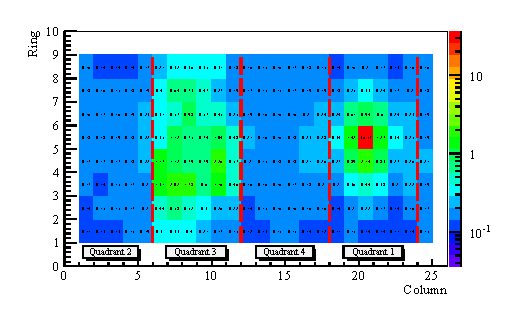
\includegraphics[width=.7\textwidth]{figures/chap4/flasher_charge_patter.eps}
	\caption{A typical flasher event with the flashing PMT in column 20 row 5 and the PMTs across the AD with high charge.}
	\label{fig:flasher_charge_pattern}
\end{figure}
To reject the flasher events, two variables are constructed, namely $MaxQ$ and $Quad$. $MaxQ$ is the largest fraction of the total detected charge seen by a single PMT. After the identification of the $MaxQ$ and the PMT corresponding to $MaxQ$, the 24 columns of PMTs are divided into four even quadrants, with the PMT with the largest charge fraction sitting in the center of the quadrant which is called Quadrant 1. Then viewed from top, the remaining quadrants are named Quadrant 2, Quadrant 3, and Quadrant 4 clockwise. The variable $Quad$ is defined as $Q_3/(Q_2+Q_4)$, where $Q_i$ is the total charge in the $i$th quadrant. It is found that the flasher events satisfy the inequality
\begin{equation}
	\left(\frac{MaxQ}{0.45}\right)^2+\left(Quad\right)^2>1
\end{equation}
The discrimination power of this cut decreases with energy. For events with values very close to $1$, careful studies are conducted, and it is found that the IBD inefficiency due to this flasher cut is $(0.02\pm 0.01)\%$~\cite{dayabay2013}. The flasher contamination in the IBD selection is estimated to be $<10^{-4}$. In addition, flasher events which survived the flasher cut would eventually be removed by the accidental background cut. Due to the high efficiency of this flasher cut, all PMTs are in operation during data taking including the flashing PMTs. In this study, all events are required to pass the flasher cut before further analysis.

\section{Data Storage and Transfer}
The raw data recorded by the DAQ system are first transferred to the Daya Bay onsite storage disks. The Performance Quality Monitoring (PQM) system~\cite{Liu2013} then uses these onsite data combined with the onsite database to produce data for online data quality check. The raw data are then transferred to the lxslc5 cluster of the Institute of High Energy Physics (IHEP) in Beijing, which in turn are transferred to the PDSF cluster of the Lawrence Berkeley National Laboratory (LBNL) for storage in the U.S.. The data route from the onsite storage to the data warehouses is shown in Figure~\ref{fig:data_transfer}.
\begin{figure}
	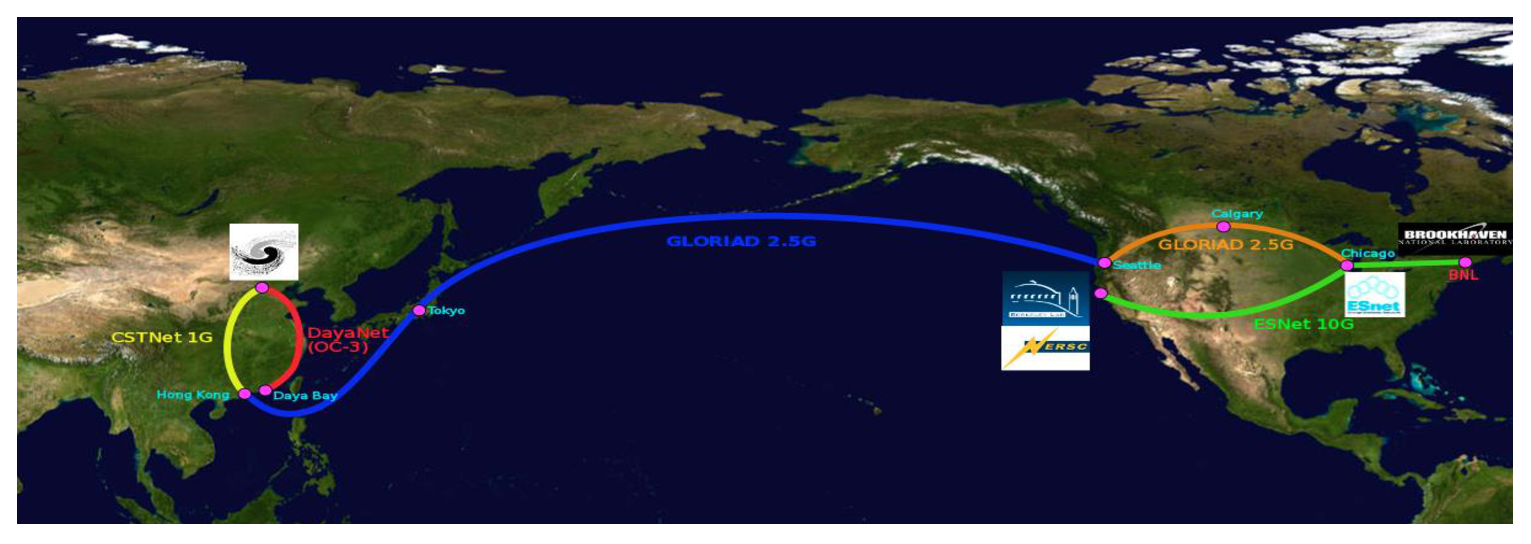
\includegraphics[width=\textwidth]{figures/chap4/data_transfer.eps}
	\caption{Data transfer from Daya Bay onsite to IHEP and from IHEP to LBNL.}
	\label{fig:data_transfer}
\end{figure}
The raw data at IHEP and LBNL are processed to produce the so called ``Keep Up Production" (KUP) data to be used by the Offline Data Monitor (ODM) system, providing offline data quality check\footnote{\href{https://portal-auth.nersc.gov/dayabay/odm}{https://portal-auth.nersc.gov/dayabay/odm}}. A Data Quality (DQ) database is constructed based on the KUP data to mark datasets with good or bad data quality.

The data transfer between the onsite and the IHEP and LBNL clusters is done with a piece of management software called SPADE. SPADE stands for South Pole Archival and Data Exchange, originally developed by IceCube and adopted by Daya Bay~\cite{docdb2696}. The design goal of SPADE is to reliably transfer data from an experiment to its data warehouse. What SPADE does is that it scans the local clusters for new files, transfers a copy to the data warehouse, and deletes the local copy. There are several advantages of employing SPADE. SPADE handles network downtime and includes bookkeeping of data movement. The adoption of SPADE by Daya Bay required only slight modifications, and SPADE has transferred Daya Bay raw data stably for years of operation.

\section{The Daya Bay Offline Software NuWa}
Daya Bay's offline software, NuWa (\textbf{N}e\textbf{u}trino at Daya \textbf{Wa}n), is a software framework~\cite{oum}. A software framework is an abstraction in which software providing specific functionality can be changed by user-written code, therefore providing application-specific software. Several key features distinguish software frameworks from libraries. The most prominent one is that the flow of control of the application is dictated by the framework instead of the user. The framework is also extensible in the sense that users can add their own code to provide specific functionality. Also the code of the framework itself is not supposed to be modified by users.

NuWa is an adaption of the LHCb/ATLAS Gaudi framework~\cite{gaudi} providing a fully developed component system for simulation, reconstruction and analysis. One important modification to Gaudi is the extension of Gaudi's Transient Event Store (TES) to Daya Bay's Archive Event Store (AES). TES is a tree (linked list) that stores all the data pertinent to the current event loop. However in the IBD analysis, not only the current event is analyzed but also the previous ones so as to form the prompt-delayed IBD coincidence. AES stores data within a user-specified time interval to resolve the problem of look-back.

Users make their own applications by writing a piece of C++ code called an ``algorithm" conforming to the requirements of the NuWa framework. Different algorithms from different authors can be cascaded to exploit the existing code. Most importantly, the adoption of software framework enables users to analyze the simulation data and the physics data with the same code.

For each data production cycle NuWa is frozen in some particular version. Before NuWa is frozen analyzers are free to add their own analysis code. After version freezing, the raw data are processed by NuWa to generate production data. The production data can be seen as ROOT trees grouped in directories. For example, the calibrated PMT hits in charge unit, the time of each PMT hit, and the RPC hit channels are all stored in the \texttt{CalibReadoutHeader} tree. The energy and vertex of each AD event, the vertex of each water pool event, and the vertex of each RPC event are reconstructed and stored in the trees in the \texttt{Rec} folder. User tagged events such as accidentals, coincidence events and muons are stored in the trees in the \texttt{Physics} folder. Table~\ref{table:production_data} lists the trees in the latest production data (P14A).
\begin{table}
	\centering
	\begin{tabularx}{\textwidth}{llX}
	\hline
	directory & tree name & use \\
	\hline
	\hline
	\texttt{\relsize{-1}/Event/CalibReadout} & \texttt{\relsize{-1}CalibReadoutHeader} & Calibrated PMT and RPC readout strip data \\
	\hline
	\texttt{\relsize{-1}/Event/Data} & \texttt{\relsize{-1}CalibStats} & Additional information for each trigger \\
	\hline
	\multirow{8}{*}{\texttt{\relsize{-1}/Event/Data/Physics}} & \texttt{\relsize{-1}ADSingles} & AD singles events outside of the muon veto window \\
	& \texttt{\relsize{-1}CoincidenceLoose} & IBD candidates with looser criteria \\
	& \texttt{\relsize{-1}CoincidenceTight} & IBD candidates with tighter criteria \\
	& \texttt{\relsize{-1}MuonData} & Muon tags \\
	& \texttt{\relsize{-1}MuonRecSimple} & Reconstructed muon track by PoolSimple and RpcSimple \\
	& \texttt{\relsize{-1}NeutronSpLoose} & Spallation neutron tags with looser criteria \\
	& \texttt{\relsize{-1}NeutronSpTight} & Spallation neutron tags with tighter criteria \\
	& \texttt{\relsize{-1}Spallation} & Muon and associated spallation neutron tags \\
	\hline
	\multirow{2}{*}{\texttt{\relsize{-1}/Event/Data/Calib}} & \texttt{\relsize{-1}Co60} & AD energy calibration data with $^{60}$Co \\
	& \texttt{\relsize{-1}Ge68} & AD energy calibration data with $^{68}$Ge \\
	\hline
	\multirow{7}{*}{\texttt{\relsize{-1}/Event/Data/Rec}} & \texttt{\relsize{-1}AdScaled} & AD energy and vertex reconstruction with $^{60}$Co \\
	& \texttt{\relsize{-1}AdSimple} & AD energy and vertex reconstruction with spallation neutrons \\
	& \texttt{\relsize{-1}AdTime} & AD vertex reconstruction with PMT timing \\
	& \texttt{\relsize{-1}AdUnfold} & AD muon track reconstruction with unfolding technique \\
	& \texttt{\relsize{-1}MuonCombined} & AD muon track reconstruction with AD PMT time and charge and RPC \\
	& \texttt{\relsize{-1}PoolSimple} & water pool vertex reconstruction with PMT charge \\
	& \texttt{\relsize{-1}RpcSimple} & RPC vertex reconstruction \\
	\hline
	\hline
	\end{tabularx}
	\caption{List of trees and uses in the production data version P14A.}
	\label{table:production_data}
\end{table}

The analysis of this study was done by writing an algorithm which fetches the geometric information of each detector and sensor (i.e. PMTs and RPC readout strips) stored in NuWa's geometric service, and uses the production data as the input data. The detailed methodology and results are presented in Chapter~\ref{chap:results}. The data analysis was done both remotely on the computing cluster at national labs and desktop computers at the University of Houston.


\subsection{Analysis on Computing Clusters}
Daya Bay has a share of the PDSF computing cluster at the National Energy Research Scientific Computing Center (NERSC)\footnote{\href{https://www.nersc.gov/}{https://www.nersc.gov/}}. PDSF is a networked distributed computing cluster designed primarily to meet the detector simulation and data analysis for large data processing projects. There are currently 2632 compute nodes available on PDSF. There is also The High Performance Storage System (HPSS)\footnote{\href{https://www.nersc.gov/users/data-and-file-systems/hpss/about/}{https://www.nersc.gov/users/data-and-file-systems/hpss/about/}} where Daya Bay stores raw and production data. The processing of the production data is done on PDSF. Any official Daya Bay collaborator has access to the CPU nodes and disk storage on PDSF.

%PDSF uses the Sun Grid Engine (SGE) as its batch system. The main instruction is \texttt{qsub}, which submits user scripts to the compute nodes in a queue until resources are granted. \texttt{qsub} can be used in array mode with a \texttt{-t} option to send a batch of similar jobs with different input at the same time. The status of a user's jobs can be checked with command \texttt{qstat}. For detailed instructions, see~\cite{SubmittingPDSFJobs}.

For a day of uninterrupted data taking, Daya Bay produces about 300 datasets of raw data. This analysis was done by sending a batch of NuWa jobs to PDSF. After processed by the user algorithm, the size of each output dataset greatly reduces from $\sim$1 GB to tens of MB. The resulting output files are then ready to undergo further analysis or generate plots.


\subsection{Analysis on Local Desktops}

High Energy Physics group at the University of Houston also has computing capacity with desktop computers with $\sim$20 cores and $\sim$20 TB storage. Since each day Daya Bay produces $\sim$300 GB of data, it is difficult to maintain a local copy of Daya Bay data more than a few days for testing analysis code. However, after data reduction on PDSF, data size is greatly reduced, and processed data can be transferred to the local computers for further analysis. The interactive jobs are much more responsive locally than remotely, and results and plots can be generated with ease locally. By this two-stage analysis method, analysis can be done efficiently, and the turnaround time between analysis iterations is shortened.